        \documentclass{standalone}
        \usepackage{../BlogTikz}
        \begin{document}

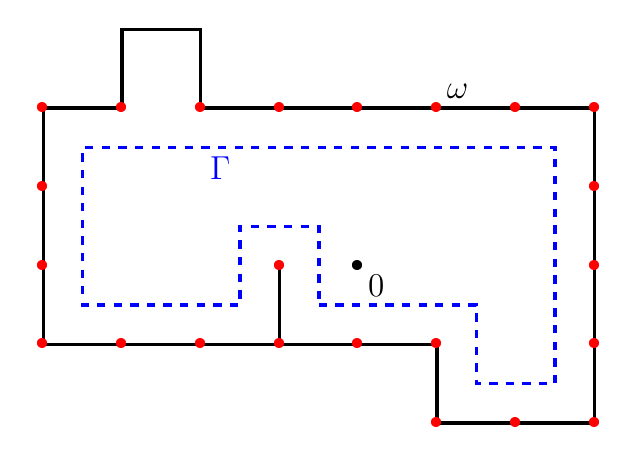
\begin{tikzpicture}[scale=1]
\tikzstyle{every node}=[font=\small]
	\node at (0,0) {\textbullet};
	\node[below right] at (0,0) {\large$0$};

	\draw[very thick, dashed, blue] (-0.5,-0.5) to (1.5,-0.5) to (1.5,-1.5) to (2.5,-1.5) to (2.5,1.5) to (-3.5,1.5) to (-3.5,-0.5) to (-1.5,-0.5) to (-1.5,0.5) to (-0.5,0.5) to cycle;
	\node[below left] at (-1.5,1.5) {\large\textcolor{blue}{$\Gamma$}};

	\draw[very thick] (-1,-1) to (1,-1) to (1,-2) to (3,-2) to (3,2) to (-2,2) to (-2,3) to (-3,3) to (-3,2) to (-4,2) to (-4,-1) to (-1,-1) to (-1,0);
	\node[above right] at (1,2) {\large$\omega$};

	\foreach \XCoord in {-4,...,1,3}{
		\foreach \YCoord in {-1,2}{
			\node at (\XCoord, \YCoord) {\textcolor{red}{\textbullet}};
		}
	}
	\node at (2,2) {\textcolor{red}{\textbullet}};
	\node at (-4,1) {\textcolor{red}{\textbullet}};
	\node at (-4,0) {\textcolor{red}{\textbullet}};
	\node at (3,1) {\textcolor{red}{\textbullet}};
	\node at (3,0) {\textcolor{red}{\textbullet}};
	\node at (1,-2) {\textcolor{red}{\textbullet}};
	\node at (2,-2) {\textcolor{red}{\textbullet}};
	\node at (3,-2) {\textcolor{red}{\textbullet}};
	\node at (-1,0) {\textcolor{red}{\textbullet}};
\end{tikzpicture}
        \end{document}
